\documentclass{article}
\usepackage{fancyhdr}
\usepackage{ctex}
\usepackage{listings}
\usepackage{graphicx}
\usepackage[a4paper, body={18cm,22cm}]{geometry}
\usepackage{amsmath,amssymb,amstext,wasysym,enumerate,graphicx}
\usepackage{float,abstract,booktabs,indentfirst,amsmath}
\usepackage{array}
\usepackage{booktabs}
\usepackage{multirow}
\usepackage{url}
\usepackage{diagbox}
\renewcommand\arraystretch{1.4}
\usepackage{indentfirst}
\setlength{\parindent}{2em}
\usepackage{enumitem}
\setmonofont{Consolas}
\usepackage{listings}
\usepackage{xcolor}
\usepackage{makecell}
\usepackage{tikz}
\usetikzlibrary{positioning, arrows.meta}
\setCJKmonofont{黑体}
\lstset{  
	% 基本设置  
	xleftmargin = 3em, xrightmargin = 3em, aboveskip = 1em,  
	backgroundcolor = \color{white},  
	basicstyle = \small\ttfamily,  
	rulesepcolor = \color{gray},  
	breaklines = true,  
	numbers = left,  
	numberstyle = \small,  
	numbersep = -14pt,  
	frame = shadowbox,  
	showspaces = false,  
	columns = fixed,  
	sensitive = true,  
	% VSCode 风格配色  
	keywordstyle = \color{blue!70!black}\bfseries,  
	emphstyle = \color{red!70!black}\bfseries, % 对于强调的词  
	emphstyle=[2]\color{purple!70!black}\bfseries, % 对于第二组强调的词  
	commentstyle = \color{green!60!black}, % 注释颜色  
	stringstyle = \color{orange!90!black}, % 字符串颜色更亮一些  
	morekeywords={ASSERT, int64\_t, uint32\_t},  
	moreemph={ASSERT, NULL},  
	moreemph=[2]{int64\_t, uint32\_t, tid\_t, uint8\_t, int16\_t, uint16\_t, int32\_t, size\_t, bool},  
	morecomment=[l][\color{green!60!black}]{+}, % 以+开头的注释  
}

%--------------------页眉--------------------%
\pagestyle{fancy}
\fancyhead[L]{}
\fancyhead[R]{}
\fancyhead[C]{华东师范大学软件工程学院}
\fancyfoot[C]{-\thepage-}
\renewcommand{\headrulewidth}{1.5pt}
%--------------------标题--------------------%
\begin{document}
\begin{center}
	{\Large{\textbf{\heiti 第十次作业——软件韧性与优雅降级}}}
	\begin{table}[H]
		\centering
		\begin{tabular}{p{2cm}p{4cm}<{\centering}p{1cm}p{2cm}p{6cm}<{\centering}}
			课程名称:    & 软件质量分析 & \quad & 指导教师:    & 陈仪香
			\\ \cline{2-2} \cline{5-5}
			姓\qquad 名: & 王海生    & \quad & 学\qquad 号: & 10235101559
			\\ \cline{2-2} \cline{5-5}
			年\qquad 级: & 2023级    & \quad & 主\qquad 题: & 软件韧性与优雅降级
			\\ \cline{2-2} \cline{5-5}
		\end{tabular}
	\end{table}
	
	% 添加新行并居中
	%\vspace{1em} % 可选:添加垂直间距
\end{center}
\rule{\textwidth}{1pt}

\tableofcontents

%--------------------正文--------------------%
\section{第一题}

\subsection{题目}

软件韧性的定义是什么,包含了哪三个可信属性和十个子属性?其定义是什么?

\subsection{解答}

\textbf{软件韧性}是指软件在遭受攻击或出现故障时,在不中断服务的情况下尽快恢复到正常工作状态的能力。通过对软件系统的韧性可信性进行评估,使软件系统满足韧性可信性需求后再进行使用,可以减少软件系统故障带来的经济损失和严重后果。

\subsubsection{软件韧性的三个可信属性}

软件韧性包含以下三个主要的可信属性:

\textbf{可生存性 (Survivability)}:系统在受到攻击、出现故障或事故的情况下,及时完成其任务的能力。
\textbf{可恢复性 (Recoverability)}:系统及时恢复其服务的能力。
\textbf{适应性 (Adaptability)}:系统调整自身或其资源以面对改变的形势或环境来维持正常工作的能力。

\begin{table}[h!]
	\centering
	\begin{tabular}{p{3cm}p{10cm}}
		\toprule
		\textbf{术语}         & \textbf{描述}                                                                 \\
		\midrule
		可生存性 (Survivability)     & 系统在受到攻击、出现故障或事故的情况下,及时完成其任务的能力。       \\
		可恢复性 (Recoverability)    & 系统及时恢复其服务的能力。                                             \\
		适应性 (Adaptability)        & 系统调整自身或其资源以面对改变的形势或环境来维持正常工作的能力。       \\
		\bottomrule
	\end{tabular}
	\caption{系统属性定义}
	\label{tab:system_properties}
\end{table}

\subsubsection{软件韧性的十个可信子属性}

每个属性下还细分为十个子属性,具体如下:

\begin{enumerate}
	\item 
	\textbf{可生存性}
	
	\begin{itemize}
		\item \textbf{可用性 (Availability)}: 在规定的时间段内系统能够按照要求运行的能力。
		\item \textbf{安全性 (Security)}: 系统保护信息和数据的能力。
		\item \textbf{容错性 (Fault Tolerance)}: 在存在包括故障、错误或攻击等威胁的情况下,系统的功能状态能够提供适当服务的程度。
	\end{itemize}
		
	\item 
	\textbf{可恢复性}
	
	\begin{itemize}
		\item \textbf{恢复性能 (Recovery Performance)}: 系统恢复其服务的能力。
		\item \textbf{恢复成本 (Recovery Cost)}: 系统在恢复过程中耗费的非时间成本。
		\item \textbf{恢复时间 (Recovery Time)}: 系统在恢复过程中涉及到的一系列时间、延时等。
	\end{itemize}
	
	\item 
	\textbf{适应性}
	
	\begin{itemize}
		\item \textbf{可拓展性 (Scalability)}: 系统可以添加新的功能。
		\item \textbf{可重配置 (Reconfigurability)}: 系统重新调整资源与进程关系的能力。
		\item \textbf{可学习性 (Learnability)}: 系统从动态环境中学习,做出适应性的决定来提高性能的能力。
		\item \textbf{自治性 (Autonomy)}: 自主控制系统在不确定环境下长时间运行良好,并在没有外部干预的情况下自动恢复系统故障的能力。
	\end{itemize}
	
\end{enumerate}

这些属性和子属性共同构成了对软件韧性全面的描述,用于评估和提升软件系统的韧性水平。

\section{第二题}

\subsection{题目}

韧性既有功能也有性能,因而既要对功能进行度量也要对性能进行度量,一般情况下,如何对其性能进行分级度量的?并以可生存性的容错性度量元定义加以说明。

\subsection{解答}

韧性既有功能也有性能,因而既要对功能进行度量也要对性能进行度量:

$$
B = \left\{ PERF^{\alpha_1} \times FUNC^{\alpha_2} \atop \alpha_1+\alpha_2 = 1 \right.
$$

\begin{itemize}
	\item PERF 为根据前表得到的性能度量值, FUNC 为根据前表得到的功能度量值, $\alpha1$ 和 $\alpha2$ 分别为性能和功能的权重, 取值范围为 [0, 1], 由专家和组件开发人员指定。
	\item 表现 B 的可信度量取值区间范围为 [1, 10]。
\end{itemize}

\subsubsection{性能的分级度量方法}

对于性能的分级度量,通常采用以下方法:

\begin{itemize}
	\item 定义性能基准:首先确定系统或组件在正常工作时的初始性能水平,作为基准。
	\item 设定度量指标:根据不同的系统或组件特性,选择合适的性能指标。例如,CPU和内存的性能可以通过工作频率来体现;屏幕的性能则可以以分辨率和触摸反馈准确率等为指标。
	\item 性能等级划分:将性能表现按照从0\%到100\%对应到1到10分的评分体系,其中10分为最高性能,1分为最低性能。
\end{itemize}

\subsubsection{以可生存性的容错性度量元定义为例}

具体到可生存性的容错性度量元定义,其度量方式如下:

\begin{enumerate}
	\item 
	\textbf{容错及其功能}:
	\begin{itemize}
		\item 如果组件对容错性有合理的测试、具有错误透明性(能给出错误根源),并且在容错阶段仍能提供服务,则该组件满足所有三项条件,获得最高评级A。
		\item 如果仅满足上述条件中的两项,则评分为B。
		\item 满足一项条件的评为C。
		\item 若不满足任何一点,则评为D。
	\end{itemize}
	
	\item 
	\textbf{容错性能}:
	\begin{itemize}
		\item 修复前平均时间(MTTF)不高于规定值;
		\item 渗透阈值(Percolation threshhold)不低于规定值;
		\item 组件与其他组件有合理的依赖关系。
		\item 当组件当前满足上述所有三点时,被评为A;满足两点为B;满足一点为C;不满足任何一点为D。
	\end{itemize}
	
	\item 
	\textbf{平均故障间隔时间(MTBF)}:
	\begin{itemize}
		\item 如果组件的平均故障间隔时间低于规定的时间,则被评为A;
		\item 如果介于规定时间的$100\%-150\%$之间,则为B;
		\item $150\%-200\%$之间为C;
		\item 超过$200\%$则为D。
	\end{itemize}
	
	\item
	\textbf{组件损失表现}:
	\begin{itemize}
		\item 组件受到攻击前后表现的变化也被用来衡量其容错能力。如果组件损失表现不超过受到攻击前表现的$10\%$,则被评为A;
		\item $10\%-40\%$之间为B;
		\item $40\%-70\%$为C;
		\item 超过$70\%$为D。
	\end{itemize}
\end{enumerate}

通过这些详细的度量标准,可以量化地评估一个组件或系统的容错能力和整体性能表现,从而确保即使在面对故障或攻击时,也能维持一定的服务水平。

\section{第三题}

\subsection{题目}

例子中的游戏系统网关组件,在客户大量增加后,性能发生了哪些变化?运行商是如何维护和解决的?解决效果如何?

\subsection{解答}

\subsubsection{客户量增大后的性能变化}

当游戏系统网关组件面临客户量大幅增加后,其性能发生了以下变化:

\begin{itemize}
	\item \textbf{可用性下降}:中国地区服务器压力剧增,导致无法提供与美国地区同等质量的服务。玩家明显感觉到延迟增加,部分玩家甚至无法连接到服务器。
	\item \textbf{服务质量受损}:对于各地区提供的服务质量,网关组件只能对超过50\%的地区提供达到质量要求的服务,而少于50\%的地区无法达到要求。
	\item \textbf{容错表现受影响}:组件损失的表现占到了受到攻击前表现的10\%-40\%,表明大约30\%的用户受到了影响,并且部分用户的影响较为轻微。
	\item \textbf{恢复性能降低}:在规定时间内,组件未能恢复损失表现的90\%以上,而是满足了损失表现30\%以下的情况。
\end{itemize}

\subsubsection{运营商采取的措施}

面对这些问题,运行商采取了如下维护和解决措施:

\begin{itemize}
	\item \textbf{增加服务器资源}:及时增加了服务器以解决由于玩家数量增加带来的服务器压力问题。
	\item \textbf{调整更新策略}:改变了更新策略,让一部分正在游玩的玩家继续游玩,未游玩的玩家才需进行更新,避免因更新导致服务器突发压力过大。
\end{itemize}

\subsubsection{问题解决效果}

解决效果评估如下:

经过上述维护措施之后,网关组件的性能得到了显著改善:

\begin{itemize}
	\item 组件再次能够向所有用户提供网络互联和游戏数据服务,非关键功能也恢复正常。
	\item 对各地区的服务质量重新达到了统一标准,即所有地区均能提供符合质量要求的服务。
	\item 容错性方面,组件损失的表现回到了不超过受到攻击前表现的10\%以内。
	\item 恢复性能方面,组件能够在规定时间内恢复损失表现的90\%以上。
	\item 适应性方面,组件添加新功能时不再影响正运行的功能,用户下次使用时只需更新即可。
\end{itemize}

最终,通过修复和升级,韧性可信度量值从灾难后的6.353恢复并提升到了8.768,这说明运营商的解决方案不仅恢复了系统的正常运作,还进一步提高了系统的韧性可信度。

\subsubsection{软件韧性的计算}

\begin{enumerate}
	\item 初始状态下的韧性可信度量值
	\begin{enumerate}
		\item \textbf{可生存性(SURV)}:
		\begin{itemize}
			\item 可用性证据权重:$0.4 \times 10 + 0.4 \times 10 + 0.2 \times 10 = 10$
			\item 安全性证据权重:$1 \times 10 = 10$
			\item 容错性证据权重:$0.3 \times 10 + 0.2 \times 10 + 0.2 \times 10 + 0.3 \times 10 = 10$
		\end{itemize}
		子属性可信值:
		$ SURV = 0.353 \times 10 + 0.324 \times 10 + 0.323 \times 10 = 10 $
		
		\item \textbf{可恢复性(REC)}:
		\begin{itemize}
			\item 恢复性能证据权重:$0.6 \times 10 + 0.4 \times 10 = 10$
			\item 恢复成本证据权重:$1 \times 10 = 10$
			\item 恢复时间证据权重:$1 \times 10 = 10$
		\end{itemize}
		子属性可信值:
		$ REC = 0.369 \times 10 + 0.294 \times 10 + 0.337 \times 10 = 10 $
		
		\item \textbf{适应性(ADAPT)}:
		\begin{itemize}
			\item 可拓展性证据权重:$0.6 \times 10 + 0.4 \times 10 = 10$
			\item 可重配置证据权重:$1 \times 7 = 7$
			\item 可学习性证据权重:$1 \times 4 = 4$
			\item 自治性证据权重:$1 \times 7 = 7$
		\end{itemize}
		子属性可信值:
		$ ADAPT = 0.251 \times 10 + 0.237 \times 7 + 0.261 \times 4 + 0.251 \times 7 = 7.481 $
		
		\item 初始韧性可信度量值 
		$ CP_{gateway} = 0.322 \times 10 + 0.410 \times 10 + 0.268 \times 7.481 = 8.321 $
	\end{enumerate}
	
	\item 故障发生后的韧性可信度量值
	\begin{enumerate}
		\item \textbf{可生存性(SURV)}:
		\begin{itemize}
			\item 可用性证据权重:$0.4 \times 7 + 0.4 \times 7 + 0.2 \times 4 = 6.4$
			\item 安全性证据权重:$1 \times 10 = 10$
			\item 容错性证据权重:$0.3 \times 7 + 0.2 \times 7 + 0.2 \times 7 + 0.3 \times 7 = 7$
		\end{itemize}
		子属性可信值:
		$ SURV = 0.353 \times 6.4 + 0.324 \times 10 + 0.323 \times 7 = 7.996 $
		
		\item \textbf{可恢复性(REC)}:
		\begin{itemize}
			\item 恢复性能证据权重:$0.6 \times 1 + 0.4 \times 1 = 1$
			\item 恢复成本证据权重:$1 \times 10 = 10$
			\item 恢复时间证据权重:$1 \times 10 = 10$
		\end{itemize}
		子属性可信值:
		$ REC = 0.369 \times 1 + 0.294 \times 10 + 0.337 \times 10 = 6.006 $
		
		\item \textbf{适应性(ADAPT)}:
		\begin{itemize}
			\item 可拓展性证据权重:$0.6 \times 1 + 0.4 \times 1 = 1$
			\item 可重配置证据权重:$1 \times 7 = 7$
			\item 可学习性证据权重:$1 \times 4 = 4$
			\item 自治性证据权重:$1 \times 7 = 7$
		\end{itemize}
		子属性可信值:
		$ ADAPT = 0.251 \times 1 + 0.237 \times 7 + 0.261 \times 4 + 0.251 \times 7 = 5.250 $
		
		\item 故障发生后的韧性可信度量值 
		$ CP_{gateway} = 0.322 \times 7.996 + 0.410 \times 6.006 + 0.268 \times 5.250 = 6.353 $
	\end{enumerate}
	
	\item 维护和解决后的韧性可信度量值
	\begin{enumerate}
		\item \textbf{可生存性(SURV)}:
		\begin{itemize}
			\item 可用性证据权重:$0.4 \times 10 + 0.4 \times 10 + 0.2 \times 10 = 10$
			\item 安全性证据权重:$1 \times 10 = 10$
			\item 容错性证据权重:$0.3 \times 10 + 0.2 \times 10 + 0.2 \times 10 + 0.3 \times 10 = 10$
		\end{itemize}
		子属性可信值:
		$ SURV = 0.353 \times 10 + 0.324 \times 10 + 0.323 \times 10 = 10 $
		
		\item \textbf{可恢复性(REC)}:
		\begin{itemize}
			\item 恢复性能证据权重:$0.6 \times 10 + 0.4 \times 10 = 10$
			\item 恢复成本证据权重:$1 \times 10 = 10$
			\item 恢复时间证据权重:$1 \times 10 = 10$
		\end{itemize}
		子属性可信值:
		$ REC = 0.369 \times 10 + 0.294 \times 10 + 0.337 \times 10 = 10 $
		
		\item \textbf{适应性(ADAPT)}:
		\begin{itemize}
			\item 可拓展性证据权重:$0.6 \times 7 + 0.4 \times 7 = 7$
			\item 可重配置证据权重:$1 \times 7 = 7$
			\item 可学习性证据权重:$1 \times 4 = 4$
			\item 自治性证据权重:$1 \times 7 = 7$
		\end{itemize}
		子属性可信值:
		$ ADAPT = 0.251 \times 7 + 0.237 \times 7 + 0.261 \times 4 + 0.251 \times 7 = 6.383 $
		
		\item 维护和解决后的韧性可信度量值 
		$ CP_{gateway} = 0.322 \times 10 + 0.410 \times 10 + 0.268 \times 6.383 = 8.768 $
	\end{enumerate}
\end{enumerate}

综上所述,通过上述计算可以清晰地看到,在灾难发生后,系统的韧性可信度量值确实下降了;而经过有效的维护和解决方案实施后,不仅恢复到了灾难前的水平,还进一步提高了系统的韧性可信度。

\section{第四题}

\subsection{题目}

软件优雅降级的目的是什么?

\subsection{解答}

\subsubsection{软件优雅降级的目的概括}

软件优雅降级的目的是在软件系统受到攻击或者内部发生故障后,通过牺牲部分性能或者功能来保证软件继续运行,而非立即停止或崩溃,从而确保系统的可靠性和稳定性,并保障系统其它部分的正常运作。

\subsubsection{软件降级及其缺点}

\textbf{软件降级}是指在软件系统中,当某个组件或模块出现问题或者为了应对新出现的需求和挑战时,将该组件或模块回退到一个较早的、被认为更加稳定或兼容性更好的版本的过程。这通常发生在二次开发过程中引入了新的程序漏洞之后,以减少因这些漏洞带来的风险。

软件降级有以下几个缺点:

\begin{enumerate}
	\item 开发和维护成本高:为系统中的每个关键组件设立一个或多个备份组件会显著增加软件系统的开发成本,并且由于系统的规模变得更大,后期的维护成本也会相应增加。
	\item 适用性有限:如果故障的原因是某个版本开发阶段遗留在组件源代码内部的程序漏洞,则简单的冗余备份机制可能无法解决问题,因为备份组件也可能包含同样的漏洞,导致它们同样不能正常运行。
	\item 功能损失:降级到早期版本可能导致失去后来添加的新功能,从而影响用户体验和服务质量。
	\item 兼容性问题:旧版本的组件可能与其他现有组件之间存在兼容性问题,这可能会引发新的错误或不稳定因素。
\end{enumerate}

\subsubsection{优雅软件降级及其优点}

\textbf{软件优雅降级}是指在软件系统受到攻击或内部发生故障后,通过牺牲部分性能或者功能来保证软件继续运行,而不是立即停止或崩溃的一种策略。它被视为一种特殊的容错机制,与传统冗余备份提升容错能力的方式不同。

软件优雅降级具有以下优点:

\begin{enumerate}
	\item \textbf{提高系统的可靠性与稳定性:} 即使在组件发生故障的情况下,系统仍能提供一定程度的服务,确保了系统的持续可用性。
	
	\item \textbf{减少开发和维护成本:} 相比为每个组件设立冗余备份的方法,优雅降级不需要额外的备份组件,从而降低了开发成本和后期维护的复杂度。
	
	\item \textbf{增强适用性:} 优雅降级不仅对由外部攻击或长时间运行导致的故障有效,而且对于因版本开发阶段遗留下来的程序漏洞所引起的故障也有效,增加了其应对各种故障场景的能力。
	
	\item \textbf{快速响应故障:} 优雅降级模型包含故障发现机制和故障隔离机制,能够及时定位故障位置,并通过隔离措施限制故障的影响范围,保障其余部分的正常运作。
	
	\item \textbf{保护用户和业务连续性:} 即使某些功能暂时受损,整个应用程序仍然可以使用,从而保持用户体验和服务水平不受严重影响。
\end{enumerate}

\section{第五题}

\subsection{题目}

优雅降级模型架构是什么?

\subsection{解答}

优雅降级模型架构是一种在系统或软件设计中采用的策略,旨在确保在部分组件或功能失效的情况下,系统仍能提供基本的功能和服务。这种架构设计的核心思想是在系统出现故障或性能下降时,通过降级某些非关键功能或服务,来维持系统的整体可用性和稳定性。

\subsubsection{流程图}

\begin{figure}[H]
	\centering
	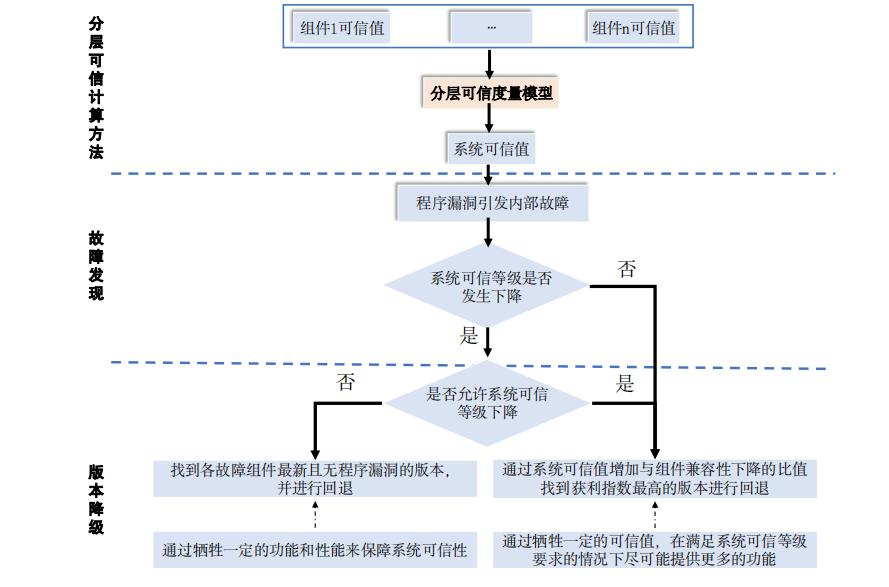
\includegraphics[width=0.9\textwidth]{img/01.png}
	\caption{优雅降级模型架构}
\end{figure}

\subsubsection{简要说明}

根据流程图,优雅降级模型架构可以分为以下几个步骤:

\begin{enumerate}
	\item \textbf{分层可信计算方法:} 首先,系统会对各个组件进行可信度评估,确定每个组件的可信值。这些可信值会输入到分层可信度量模型中,计算出系统的整体可信值。
	
	\item \textbf{故障发现:} 系统会持续监控各个组件的状态,一旦发现某个组件出现故障或可信度下降,会触发故障发现机制。
	
	\item \textbf{系统可信等级是否下降:} 系统会判断当前的故障是否导致了系统整体可信等级的下降。如果系统可信等级下降,则进入下一步;如果未下降,则继续监控。
	
	\item \textbf{是否允许系统可信等级下降:} 系统会判断是否允许当前的可信等级下降。如果允许,则进入版本降级步骤;如果不允许,则会尝试通过其他方式恢复系统可信等级。
	
	\item \textbf{版本降级:} 如果允许系统可信等级下降,系统会选择一个较低版本的组件进行回退,以牺牲一定的功能和性能来保障系统的整体可用性和稳定性。
	
	\item \textbf{通过牺牲一定的功能和性能来保障系统可用性:} 在版本降级后,系统会牺牲一定的功能和性能,以确保系统的基本功能和服务能够继续运行。
	
	\item \textbf{通过牺牲一定的可信值,在满足系统可信等级要求的情况下尽可能提供更多的功能:} 在系统可信等级允许的情况下,系统会尽可能提供更多的功能,以满足用户的需求。
\end{enumerate}

通过这种优雅降级模型架构,系统能够在部分组件或功能失效的情况下,仍然保持基本的可用性和稳定性,从而提高系统的整体可靠性。

\section{第六题}

\subsection{题目}

当软件系统发生故障后,可信等级已经发生了下降,但不允许可信等级发生下降的情况下如何选择组件的版本?

\subsection{解答}

当软件系统发生故障导致可信等级下降且不允许此下降时,需通过\textbf{定位故障组件}并采用\textbf{二分搜索算法}确定各组件的最佳回退版本,以最小化回退成本和恢复系统的可信度。随后,基于\textbf{分支定界法}选择最优的故障组件进行版本回退,确保系统满足其可信等级要求。

\subsubsection{故障定位}

\begin{enumerate}
	\item 
	\textbf{监控系统可信值变化:} 参照基于组件的分层可信计算模型,实时计算软件各层的可信值,建立组件、功能模块、服务、子系统以及系统的可信值与时间的关系,并实时监控系统可信值。当系统可信值下降时,判断系统内部发生故障。
	
	\item
	\textbf{确定故障子系统、服务和功能模块:} 根据各子系统的可信值变化情况判断存在故障组件的子系统,再自上而下依次检查各服务和各功能模块的可信值变化情况,进一步细化故障位置。
	
	\item 
	\textbf{定位故障组件:} 查看各组件的可信值下降情况及变化原因,判断组件是否遭受故障传播影响,并结合下降原因确定故障源,完成故障组件定位。
\end{enumerate}

\subsubsection{确定组件回退版本(以用户验证组件为例)}

采用\textbf{二分搜索}算法思想,不断缩小搜索区间,通过重新度量对应版本的组件可信度,直至找到最优回退版本。例如,用户验证组件存在 8 个版本,经过 3 次区间缩小及重新度量,最终确定其最佳回退版本为 V1.3.0。

\subsubsection{计算各故障组件回退版本的相关信息(四元组信息)}

包括最佳回退版本、回退成本(通过基于组件版本号的成本函数计算,考虑组件版本回退导致的兼容度下降程度等因素)、系统可信度上升情况等。例如:

\begin{itemize}
	\item 用户验证组件:最佳回退版本为 V1.3.0,回退成本为 $5.3\times10^{-3}$,系统可信度上升情况为 0.133。
	\item 隐私设置组件:最佳回退版本为 V1.2.2,回退成本为 $4.3\times10^{-3}$,系统可信度上升情况为 0.034。
\end{itemize}

\subsubsection{选择故障组件及版本回退方案}

\begin{enumerate}
	\item 
	\textbf{选择故障组件选择算法:} 结合软件系统的可信要求,因系统不允许可信等级下降,选择\textbf{基于分支定界法的故障组件选取算法}。
	
	\item 
	\textbf{确定组件版本回退方案:} 接入分层可信度量工具实时计算系统和子系统的可信值,判断组件选取方案是否满足系统可信要求。例如在课件的例子中,最终确定如用户验证组件回退至 V1.3.0、隐私设置组件回退至 V1.8.0、订单确认组件回退至 V1.7.1、电影搜索组件回退至 V1.6.0 等方案,此时系统可信等级满足 5 级可信,花费总成本最少为 $1.59\times10^{-2}$。
\end{enumerate}

\end{document}